\documentclass[letterpaper]{article} % DO NOT CHANGE THIS
\usepackage{aaai2027}  % DO NOT CHANGE THIS
\usepackage[hyphens]{url}  % DO NOT CHANGE THIS
\usepackage{graphicx} % DO NOT CHANGE THIS
\urlstyle{rm} % DO NOT CHANGE THIS
\def\UrlFont{\rm}  % DO NOT CHANGE THIS
\usepackage{natbib}  % DO NOT CHANGE THIS AND DO NOT ADD ANY OPTIONS TO IT
\usepackage{caption} % DO NOT CHANGE THIS AND DO NOT ADD ANY OPTIONS TO IT
\frenchspacing  % DO NOT CHANGE THIS
\setlength{\pdfpagewidth}{8.5in} % DO NOT CHANGE THIS
\setlength{\pdfpageheight}{11in} % DO NOT CHANGE THIS
\usepackage{booktabs}
\usepackage{tikz}
\usetikzlibrary{positioning,arrows.meta}
\pdfinfo{
/TemplateVersion (2027.1)
}
\setcounter{secnumdepth}{0}

% TBD marks results from runs still in progress (2026-09-26). Remove before submission.
\newcommand{\tbd}{\textbf{TBD}}

\title{ForeSight: Small Calibrated Decision Models as Opponent Forecasters\\for Lookahead Game Play (Student Abstract)}
\author{
    Saiakhil Chilaka
}
\affiliations{
    Cornell University\\
    sc3484@cornell.edu
}

\begin{document}

\maketitle

\begin{abstract}
Choosing well against an opponent requires forecasting how the opponent will respond. Hand-built game engines forecast with expert rules and exact simulators, which do not exist for less deterministic settings such as negotiation, while LLM agents forecast with large generative models that are slow and poorly calibrated. We propose ForeSight, which fine-tunes a small non-generative ``System One'' decision model to output a calibrated probability for each opponent action, and uses these forecasts to weight every branch of a lookahead search. In Pok\'emon Showdown, a 421M-parameter forecaster fine-tuned for 35 minutes on a laptop, using only low-quality bot games, predicts the opponent's next action with 72--80\% accuracy (versus 43\% zero-shot and 49\% for a damage-based rule), and 75\% on an opponent it never saw in training, at 36--84\,ms per forecast. Without any LLM, ForeSight wins 56.5\% of 200 games against the Abyssal benchmark bot, on par with the LLM agent PokéLLMon (56\%), though below PokéChamp (64--70\%). Because every component is still minimal, these results suggest substantial headroom for small calibrated forecasters to bring engine-style lookahead where engines cannot be hand-written.
\end{abstract}

% Code --- add the public repository link here before submission.

\section{Introduction}
Many decisions, from game moves to negotiation offers, are only as good as the agent's forecast of how the other side will react. Classical game engines make these forecasts with search over an exact simulator and an expert-written evaluation; the Pok\'emon engine Foul Play pairs tree search with a hand-tuned position score \citep{foulplay}. This works where the rules are fully specified, but it does not transfer to settings such as negotiation, where there is no simulator and no obvious way to hand-write an opponent model.

LLM agents take the opposite route. PokéLLMon prompts an LLM to choose each move \citep{pokellmon}, and PokéChamp uses an LLM to sample actions, model the opponent and score positions inside a minimax search \citep{pokechamp}. LLMs bring broad knowledge, but each call takes seconds, their stated probabilities are poorly calibrated, and PokéChamp attributes about a third of its losses to running out of turn time.

To overcome these challenges, we propose ForeSight. Unlike prior approaches, ForeSight separates \emph{forecasting} from \emph{deciding}: a small System One decision model \citep{jev,laya}, which reads a state and a set of typed options and returns calibrated probabilities in a single forward pass without generating text, forecasts the opponent, and a probability-weighted search turns those forecasts into a decision.

\section{ForeSight}
ForeSight has three components (Figure~\ref{fig:overview}).

\begin{figure}[t]
\centering
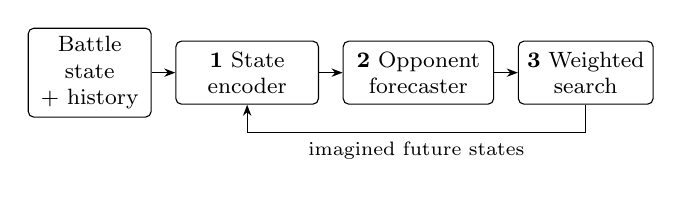
\begin{tikzpicture}[font=\footnotesize, node distance=3mm,
  box/.style={draw, rounded corners=2pt, align=center, inner sep=3pt, minimum height=8mm},
  arr/.style={-{Stealth[length=4pt]}}]
\node[box, text width=1.35cm] (s) {Battle state\\+ history};
\node[box, text width=1.6cm, right=of s] (e) {\textbf{1} State\\encoder};
\node[box, text width=1.7cm, right=of e] (f) {\textbf{2} Opponent\\forecaster};
\node[box, text width=1.5cm, right=of f] (x) {\textbf{3} Weighted\\search};
\draw[arr] (s) -- (e);
\draw[arr] (e) -- (f);
\draw[arr] (f) -- (x);
\draw[arr] (x.south) -- ++(0,-3.5mm) -| node[pos=0.25, below, font=\scriptsize]{imagined future states} (e.south);
\end{tikzpicture}
\caption{ForeSight. The forecaster assigns a probability to each opponent action; the search weights every imagined future by these probabilities and by chance, then picks the best expected move.}
\label{fig:overview}
\end{figure}

\textbf{1. State encoder.} Each position is rendered as short precomputed facts rather than raw text: remaining units and HP, which side moves first, estimated damage and knock-out chances for each attack, type effectiveness, and both sides' last few actions. Candidate opponent actions are the revealed moves, one placeholder attack per type for unrevealed moves, and switches to seen Pok\'emon.

\textbf{2. Opponent forecaster.} We fine-tune Laya \citep{laya}, an open 421M-parameter System One model, on 10k opponent decisions sampled from 142k logged in local battles between simple rule-based and random bots, a deliberately low-quality data source. We update the top four encoder layers and the decision head (75M parameters) with Laya's proper-scoring-rule objective and fit a temperature on validation data. Training takes 35 minutes on an Apple M5 laptop.

\textbf{3. Probability-weighted search.} ForeSight runs a depth-2 expectimax. For each of our actions it branches over the forecaster's opponent distribution and over chance outcomes (accuracy, damage rolls near a knock-out, secondary effects, speed ties), pruning each node to 90\% of its probability mass. Leaf positions are scored by remaining-HP balance, and the action with the highest expected value is played.

\section{Evaluation}
\textbf{Experimental Setup.} We evaluate Gen 9- and Gen 8-trained forecasters on held-out battles, against a rule favoring the opponent's strongest attack. For play, we follow PokéChamp's protocol: Gen 8 random battles without Dynamax against the rule-based Abyssal bot, which never appears in our training data, on a local Showdown server with a 15\,s turn limit. We compare with the win rates published by \citet{pokechamp}.

\begin{table}[t]
\centering
\small
\begin{tabular}{llcc}
\toprule
Forecaster & Evaluated on & Acc. & Log-loss \\
\midrule
Damage-based rule & Gen 9 bots & 48.5\% & 1.24 \\
Laya, zero-shot & Gen 9 bots & 43.4\% & 1.15 \\
ForeSight (Gen 9) & Gen 9 bots & 71.8\% & 0.70 \\
ForeSight (Gen 8) & Gen 8 bots & \textbf{79.6\%} & \textbf{0.54} \\
\midrule
ForeSight (Gen 9) & Abyssal, unseen & 73.0\% & 0.62 \\
ForeSight (Gen 8) & Abyssal, unseen & 75.4\% & 0.58 \\
\bottomrule
\end{tabular}
\caption{Next-action forecasting on held-out turns ($n{=}$3,754--4,000 bot turns; 1,963 Abyssal turns).}
\label{tab:forecast}
\end{table}

\begin{table}[t]
\centering
\small
\begin{tabular}{llc}
\toprule
Agent & Decision model & Win rate \\
\midrule
PokéLLMon$^\dagger$ & GPT-4o & 56\% \\
PokéChamp$^\dagger$ & Llama-3.1-8B & 64\% \\
PokéChamp$^\dagger$ & GPT-4o & 70\% \\
\midrule
ForeSight (Gen 9) & Laya 421M & 56.5\% \\
ForeSight (Gen 8) & Laya 421M & 56.5\% \\
\bottomrule
\end{tabular}
\caption{Win rate against Abyssal. $^\dagger$Published by \citet{pokechamp}. ForeSight: $n{=}200$ games each, 95\% CI 50--63\%.}
\label{tab:play}
\end{table}

\textbf{Forecasting.} Fine-tuning turns a weak zero-shot model into an accurate, well-calibrated forecaster (calibration error 0.02; Table~\ref{tab:forecast}) that transfers to Abyssal, never seen in training, predicting 73--75\% of its actions.

\textbf{Play.} With no LLM, ForeSight performs on par with PokéLLMon while using a model a fraction of its size, though below PokéChamp (Table~\ref{tab:play}). The Gen 8 forecaster predicts better yet wins at the same rate; since forecasts on Abyssal are already accurate, the gap to PokéChamp likely lies more in our shallow search and simple leaf.

\textbf{Speed and depth.} A forecast costs 36--84\,ms depending on batch size, and a turn takes 2.7--4.1\,s on average (about 15 forecasts and 73 search nodes), so the 15\,s budget would allow 10--25$\times$ more search than we use. Depth pays off: with a fixed rule-based forecaster, win rate against a heuristic bot rises from 56\% to 61\% to 66\% at depths 1--3 ($n{=}200$ each). The idea also extends beyond games: in the text household benchmark ALFWorld \citep{alfworld}, letting a System One model choose among an LLM's top three actions by predicted outcome raised success from 34.6\% to 48.4\% ($p{<}0.001$).

\section{Conclusion and Future Work}
We proposed ForeSight, which uses a small, fine-tuned, calibrated decision model as the opponent forecaster inside a lookahead search. Even in this deliberately minimal form, it matches an LLM agent built on a much larger model. Zero-shot System One models (Laya, and Jev in our pilots) were weak forecasters, so domain fine-tuning is essential.

\textbf{Headroom.} Every component was kept simple, and each has a clear path to improvement backed by our results:
(1)~\emph{Deeper search}: we use under a tenth of the turn budget, and win rate grew with every added level of depth.
(2)~\emph{Better data}: the forecaster was trained only on weak bot games yet already predicts an unseen opponent 75\% of the time; replays of high-rated human games \citep{metamon} should sharpen it further.
(3)~\emph{A learned leaf}: positions are scored by HP alone, so a setup move such as Swords Dance counts only if its extra damage lands within two turns; a learned win-probability leaf can value boosts, status and hazards.
(4)~\emph{Full fine-tuning and exact rules}: we updated only 18\% of the parameters, and an exact engine \citep{pokeengine} with sampled hidden teams would remove known simulator errors.
Because forecasts on Abyssal are already accurate, we expect (1), (3) and (4) in particular to narrow the gap to PokéChamp. Beyond games, ForeSight needs no hand-written opponent model, so we will extend it to negotiation \citep{dealornodeal}, where an LLM proposes candidate next states and the forecaster weighs them.

\bibliography{refs}

\end{document}
